\chapter{Parallel Implementation}
The parallel implementation consists of two applications.
\par
A server that is used to facilitate communication between all the clients and to provide the graphical user interface to interact with all the clients.
\par
A client that is used to generate the solution for the traveling salesman problem using a genetic algorithm. The client will also communicate with the server to get information about the other clients results.
\newline
The actions that are available through the server:
\begin{itemize}
  \item You can visualize the solution on a graph.
  \item Start\textbackslash Stop the work on all clients connected.
  \item Switch the instance of the problem to be solved by the clients.
  \item Export the solution.
\end{itemize}
\bigskip
The actions that are available through the client:
\begin{itemize}
  \item You can select the number of processes to be started.
  \item Connect and receive work from the server.
  \item Updating the population of the genetic algorithm from the server using migration.
\end{itemize}
\bigskip

\section{Technologies used}
\subsection{Python}
Python\footnote{Python \url{https://www.python.org}} is an object-oriented, interpreted programming language.
Modules, exceptions, dynamic typing, very high level dynamic data types, and classes are all included.
\par
I chose the Python programming language because of its versatility, efficiency, reliability, and extensive support libraries. It is also portable across operating systems.
\par
One of the main concerns and disadvantages of using Python is the Global Interpreter Lock (GIL). GIL is a mutex (or a lock) that allows only one thread to hold control of the Python interpreter. This will make our parallel algorithm redundant when run on a single system. I overcame the limitation of the GIL by using multiple processes instead of threads.
\subsection{Package Installer for Python (PIP)}
Package Installer for Python\footnote{PIP \url{https://pypi.org/project/pip/}} is a package manager written in Python and is used to install and manage software packages. It hosts thousands of third-party modules for Python.
\par
PIP was used to obtain the library for the graphical user interface and its addons.
\subsection{PySide2}
PySide2 \footnote{PySide2 \url{https://pypi.org/project/PySide2/}} is the official Python module from the Qt for Python project, which provides access to the complete Qt 5.12+ framework.
\par
I chose PySide2 because Qt is a reliable, fast, and easy-to-use graphical user interface framework. It is also cross-platform.
\subsection{GitHub}
GitHub is a provider of Internet hosting for software development and version control using Git. The source code of this project is hosted on Github. I chose Github because it satisfies the requirements of my project.
\newpage
\section{Server}
\subsection{Graphical user interface}
\begin{figure}[ht]
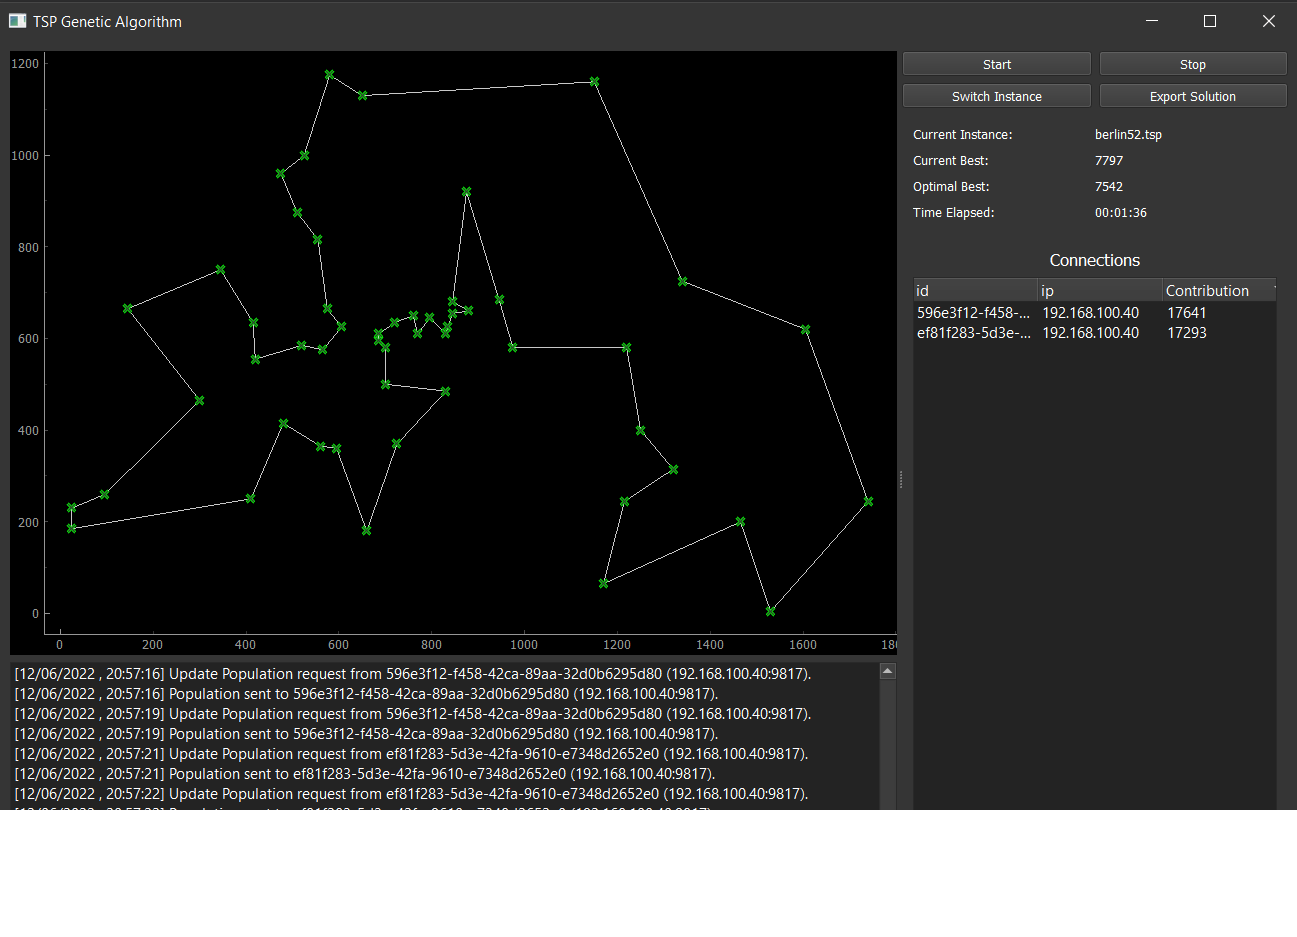
\includegraphics[width=\textwidth]{images/gui.png}
\caption{Graphical user interface}
\end{figure}
\noindent
The graphical user interface consists of the following:
\begin{enumerate}
  \item A window to visualize the current best solution found.
  \item A console with the latest logs.
  \item A menu that allows the user to control the clients (Start\textbackslash Stop, Switch instance, Export solution buttons).
  \item A section that shows information about the current instance (current instance, current best, optimal best, time elapsed).
  \item A list of currently active connections with the server.
\end{enumerate}
\clearpage
\subsection{Architecture}
\begin{figure}[ht]
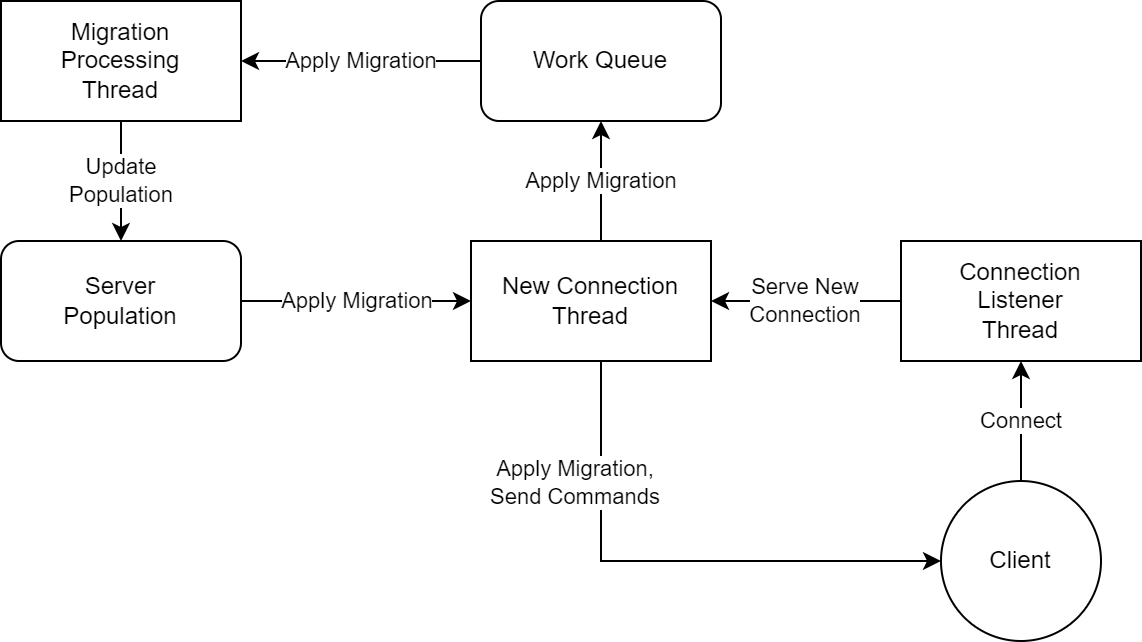
\includegraphics[width=\textwidth]{images/server_architecture.png}
\caption{Server architecture}
\end{figure}
The server architecture consists of 3 main threads: the GUI thread, which is used to process the graphical user interface; the connection listener thread, which is used to serve new connections; and the migration processing thread, which is responsible for performing migration with the data received from the clients.
\subsection{Connection listener thread}
The connection listener thread is responsible for the initial communication with the client and the spawning of a new thread to service the new connection.
\newline
Possible communication messages are:
\begin{itemize}
  \item Connect
  \item CloseConnection
  \item CloseServer
\end{itemize}
\newpage
When a "Connect" message is received, it spawns a new thread. The new thread lives while the new connection is active and is used to serve the client with the following communication messages:
\begin{itemize}
  \item GetWork
  \item UpdatePopulation
  \item CloseConnection
\end{itemize}
\par
When receiving "GetWork" from the client, the server will either send the current instance and its parameters to the client or it will send the "Stop" message based on its current work state.
\par
When receiving "UpdatePopulation" from the client, the server will perform a migration with the client if the instance is the same one. If the instance has changed since the client work has started, the server will send the "ChangeInstance" message to update the client to the current instance.
\subsection{Migration processing thread}
The migration processing thread is responsible for managing the population on the server that is used for migration. When a new client sends "UpdatePopulation", its current population is put in a work queue to be processed by the migration processing thread, and the server population is sent to perform migration. This work queue is of the Last-In-Last-Out (LILO) type, so that in the event of the thread getting overwhelmed with work, it will process new and improved populations first and be able to skip old and irrelevant populations.
\newpage
\section{Client}
The client has no graphical user interface and is only available through the command line. You are able to provide it with the number of processes to spawn. Each process spawned has its own connection with the server. By using a multiprocessing approach instead of a multithreaded one, we avoided being CPU-bound by the Python global interpreter lock.
\subsection{Architecture}
The client architecture is the same as the one described in chapter 2.3 except for the added functionality to be able to communicate with the server outside of migration.
\newline
The main loop of the clients consists of the following:
\begin{lstlisting}[language=Python]
def start(self, ip, port):
    self.initConnection(ip, port)
    while True:
        p, Chromosome_Size, Coordinates = self.getWork()
        if p:
            self.file = p[7]
            self.GA(*p,Chromosome_Size,Coordinates)
        time.sleep(2)
\end{lstlisting}
At the beginning the client will initialize a connection with the server. This is done by sending the message "Connect" to the server in self.InitConnection(ip, port). Afterwards we keep trying to get work from the server every few seconds until we receive some parameters to start the genetic algorithm.
\par
Then the genetic algorithm will perform migration for every new solution that is better than the last for a faster convergence at the beginning or after every $N$ generations.
\par
When performing migration the client sends to the server the message "UpdatePopulation" and can receive from the server the following:
\begin{itemize}
  \item Migration
     \begin{itemize}
        \item If it receives "Migration" from the server that means the migration was accepted and its ok to perform it on the client side as well.
     \end{itemize}
  \item ChangeInstance
   \begin{itemize}
    \item If it receives "ChangeInstance" from the server it means that the instance has changed on the server and the client is required to do so as well. It will then proceed to restart the genetic algorithm with the new parameters.
    \end{itemize}
  \item Stop
     \begin{itemize}
    \item If it receives "Stop" it will stop the current genetic algorithm from running.
    \end{itemize}
\end{itemize}

\newpage
\section{Performance}
To evaluate the performance of the algorithm, I ran the program on the TSP map \emph{berlin52.tsp} for 60 seconds, 15 times with the same parameters for each number of processes. The optimal solution for this map is 7542.
\newline
The results were obtained after running on the following configuration:
\begin{itemize}
    \item Operating System: Windows 10
    \item Processor: AMD Ryzen 5 1600 (3.2 GHz)
    \item Memory: 16 GB
\end{itemize}

\begin{figure}[ht]
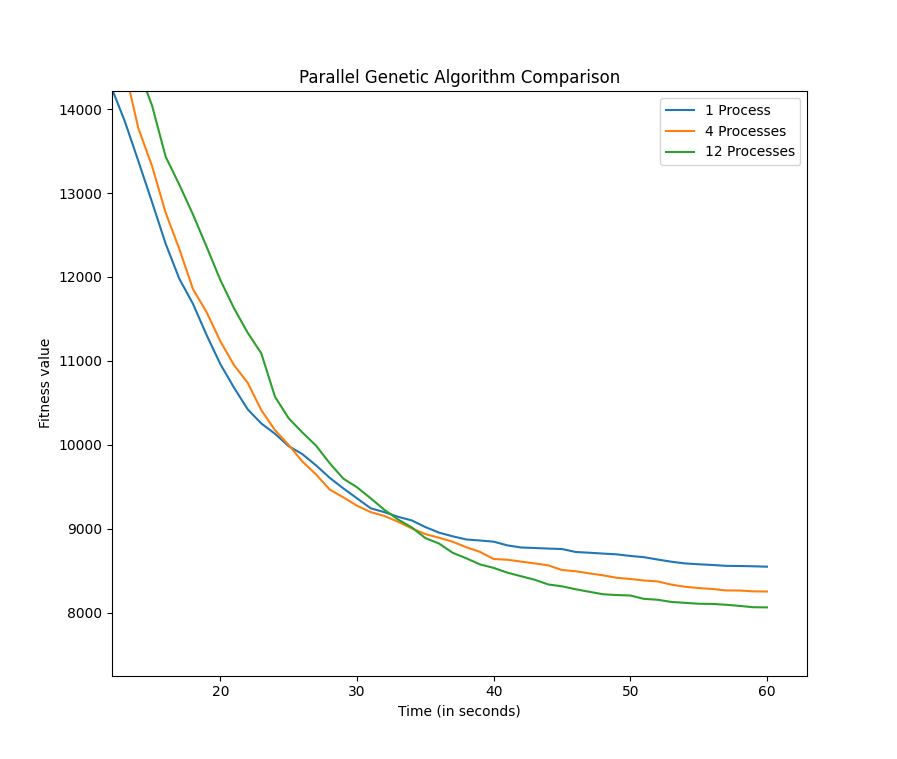
\includegraphics[width=\textwidth]{images/results.png}
\caption{Number of processes comparison}
\end{figure}
\newpage
\noindent
From the graph in Figure 3.3 we can observe two things:
\begin{itemize}
    \item For the first 30 seconds, the fewer the number of processes, the better the results.
    \item After the first 30 seconds, it's the exact opposite; the higher the number of processes, the better the results.
\end{itemize}
\par
The first point can be explained by the communication overhead generated by the migration function. We call the migration function every time we find a better solution on a client. This results in a lot of calls to the server, which in turn slows it down until the solutions stop converging so fast.
\par
From the second point it results that there is a relation between the number of processes and the solution found.
\newline
 \begin{longtable}[c]{| c | c |}
 \caption{Average of the final values after 60 seconds.\label{long}}\\
 \hline
 K-Processes & Fitness value\\
 \hline
 \endfirsthead

 \hline
 \multicolumn{2}{|c|}{Continuation of Table \ref{long}}\\
 \hline
 K-Processes & Fitness value\\
 \hline
 \endhead

 \hline
 \endfoot

 1 Process & 8550\\
4 Processes & 8254\\
 12 Processes & 8065\\
 \hline
 Optimal Solution & 7542\\
 \end{longtable}
Because genetic algorithms are metaheurisitc and use some form of stochastic optimization, they do not guarantee that a globally optimal solution can be found. Because of this, we cannot easily calculate the speedup achieved by a parallel algorithm. But from the results in Table 3.1 and Figure 3.3, we can conclude that there is an increase in performance with the increase in the number of processes.